\documentclass[twocolumn]{article}
\usepackage{xeCJK}  %必须加xeCJK包
\setCJKmainfont{AR PL UMing CN}  %换成本地字体

\usepackage{times}
\usepackage{graphicx} % more modern
\usepackage{epstopdf}
\usepackage{subfigure} 
\usepackage{natbib}
\usepackage[boxed]{algorithm}
\usepackage{algorithmic}
%\usepackage{hyperref}
\usepackage{framed}
\newcommand{\theHalgorithm}{\arabic{algorithm}}
\usepackage{tikz} %加水印用
\usepackage{eso-pic}

\usepackage{amsmath}
\usepackage{array}
\usepackage{stackengine}

\usepackage[letterpaper, margin=1in, top=0.5in]{geometry}
\usepackage[unicode]{hyperref}


\newcommand\BackgroundPicture{%
  \put(0,0){%
    \parbox[b][\paperheight]{\paperwidth}{%
      \vfill
      \centering%
        \begin{tikzpicture}[remember picture,overlay]
        \node [rotate=60,scale=8,text opacity=0.15] at (current page.center)
        { 七月在线翻译组       %\copyright XXX Powered by~\LaTeX
        };
        \end{tikzpicture}%
%      \vfill
    }}}

\begin{document}


\newcommand{\jac}[2]{\frac{\partial #1}{\partial #2}}
\newcommand{\xhat}{\widehat{x}}
\newcommand{\yhat}{\widehat{y}}
\newcommand{\zhat}{\widehat{z}}
\newcommand{\vxhat}{\widehat\mathrm{x}}
\newcommand{\vzhat}{\widehat\mathrm{z}}
\newcommand{\setX}{\mathcal{X}}
\newcommand{\setB}{\mathcal{B}}
\newcommand{\E}{\text{E}}
\newcommand{\Var}{\text{Var}}
\newcommand{\Cov}{\text{Cov}}
\newcommand{\Fhat}{\widehat{F}}
\newcommand{\Thetahat}{\widehat{\Theta}}
\newcommand{\Norm}{\text{Norm}}
\newcommand{\BatchNorm}{\text{BN}}
\newcommand{\kk}{{(k)}}
\newcommand{\vx}{\mathrm{x}}
\newcommand{\vy}{\mathrm{y}}
\newcommand{\vz}{\mathrm{z}}
\newcommand{\vb}{\mathrm{b}}
\newcommand{\vu}{\mathrm{u}}
\newcommand{\comt}{// }
\renewcommand{\algorithmiccomment}[1]{\comt #1}
\newcommand{\BN}[2]{\text{BN}_{#2}(#1)}
\renewcommand{\algorithmicrequire}{\textbf{Input:}}
\renewcommand{\algorithmicensure}{\textbf{Output:}}
\newcommand{\mils}{\cdot 10^6}
\newcommand{\netw}[1]{{\sl #1}}
\newcommand{\norig}{\text{\sl N}}
\newcommand{\ntrain}{\norig_\mathrm{BN}^\mathrm{tr}}
\newcommand{\ninf}{\norig_\mathrm{BN}^\mathrm{inf}}
\setcitestyle{authoryear,round,citesep={;},aysep={,},yysep={;}}
\renewcommand{\cite}[1]{\citep{#1}}

\title{批量规范化:通过减少内部协变量转移加速深度网络训练}

\author{Sergey Ioffe \\Google Inc., {\sl sioffe@google.com} \and
Christian Szegedy \\Google Inc., {\sl szegedy@google.com} \and 翻译:Kenny(初),管枫(复),任远航(审)\\
\href{https://github.com/JulyEdu-PaperTranslation/DeepLearning}{七月在线翻译组}
}

\date{}

\maketitle

\begin{abstract}

在深度神经网络的训练过程中,先前层参数的调整会导致之后每一层输入值的分布发生变化,这种现象使模型的训练变得很复杂.所以在深度神经网络模型的训练中,通常需要仔细选取初始参数并采取较小的学习率,这不但导致模型训练的效率低下,而且使得饱和非线性模型的训练极为困难. 我们把这种现象称为内部协变量转移({\em
  internal covariate shift}),并通过规范化(normalizing)每层的输入来解决这个问题.  
我们方法的强大之处在于把规范化的步骤作为模型训练架构的一部分来实现, 并且对每个{\em 训练小批量}都执行规范化操作.
批量规范化允许我们使用很高的学习率并且对初始化不太在意.它在一定情况下也可以起到正则化的作用,并减轻了对Dropout的需求.我们在最先进的图像分类模型中使用批量规范化法,在减少了14倍训练步骤的情况下实现了与原模型相同的精度,并以显著增量击败了原始模型.我们使用批量规范化的网络模型,增强了在ImageNet分类上发布的最佳结果:获得了4.9\%前5验证误差(和4.8\%测试误差),这超出了人类评估者的准确率
\end{abstract}

\AddToShipoutPicture{\BackgroundPicture}

\section{Introduction}

深度学习极大地提升了视觉,语言和许多其他领域。随机梯度下降(SGD)已经被证明是训练神经网络的一个有效的方法,并且随机梯度下降变种方法如动量\cite{momentum}和Adagrad\cite{momentum}已经被用来获得最先进的性能。随机梯度下降优化网络的参数$\Theta$,以便最小化损失
$$\Theta = \arg \min_\Theta
\frac{1}{N}\sum_{i=1}^N \ell(\vx_i, \Theta)$$
其中$\vx_{1\ldots N}$是训练集。在训练的每一步中我们考虑一个大小为$m$的小批量。这个小批量被用来近似相关联参数的损失函数的梯度,通过计算
$$\frac{1}{m} \jac{ \ell(\vx_i, \Theta)}{ \Theta}.$$
使用小批量的样本,而不是一次一个样本,有几点好处。首先,小批量上的损失梯度是训练集上梯度的一个估计,其质量随着批量大小的增加而提高。第二,由于现代计算平台提供的并行性,对一个批量$m$的计算比每个样本的$m$次计算更有效

虽然随机梯度是简单有效的,但是它需要仔细调整模型超参数,特别是使用在优化中的学习率以及模型参数的初始值。由于每层的输入受所有先前层的参数影响的事实,使训练复杂化,以致于网络参数的小变化随着网络变得更深而放大。

由于层需要不断地适应新的分布,层输入的分布的变化提出了一个问题。当一个学习系统的输入分布改变时,也就认为经历了{\em 协变量移位}\cite{covariate-shift},这个通常通过域适应(domainadaptation)\cite{domain-adaptation-survey}来处理。
但是,协变量移位的概念可以作为一个整体延伸超出学习系统,适用于他自身的部分,比如子网络或者一个层。
设想一个计算如下损失函数的网络:$$\ell = F_2(F_1(\vu, \Theta_1), \Theta_2)$$ 其中
$F_1$ 和 $F_2$ 可以是任意变换, 网络通过训练参数
$\Theta_1, \Theta_2$ 来最小化损失函数 $\ell$.
对 $\Theta_2$ 的学习可以被看做以
$\vx=F_1(\vu,\Theta_1)$ 为输入,以
$$\ell = F_2(\vx, \Theta_2).$$ 为损失函数的独立网络。比如,梯度下降步骤
$$\Theta_2\leftarrow \Theta_2 - \frac{\alpha}{m}\sum_{i=1}^m
\jac{F_2(\vx_i,\Theta_2)}{\Theta_2}$$ (批量大小为 $m$ 学习率
为 $\alpha$) 完全等同于一个输入为$F_2$的独立网络$\vx$.  
因此,输入分布的属性使得训练更有效 -- 比如在训练和测试数据之间有相同的分布 -- 也适用于子网络的训练。
因此有利于$\vx$的分布随时间保持不变,同时$\Theta_2$不必不断调整来适应$\vx$分布的变化.

固定一个子网络输入的分布将对子网络外的层产生积极的影响。
用一个sigmoid激活函数$\vz = g(W\vu+\vb)$考虑一个层,其中$\vu$是层输入,权重矩阵$W$和阈值向量$\vb$是学习的层参数,$g(x) = \frac{1}{1+\exp(-x)}$。
随着$|x|$ 增加,$g'(x)$ 趋向于0.这意味着对于$\vx=W\vu+\vb$的所有维度,除了那些具有小的绝对值的,梯度流向下到$\vu$会消失并且模型训练会变慢。
但是因为$\vx$是受$W, \vb$和下面所有层参数的影响,在训练期间对这些参数的改变将可能将$\vx$的许多维度移动到非线性的饱和状态并且收敛减慢。
这种效果是随着网络的深度的增加而放大的。
在实际应用中,饱和问题(saturationproblem)和导致的消失梯度通常通过使用Rectified Linear Units(ReLU)\cite{relu} $ReLU(x)=\max(x,0)$,细致的初始化\cite{glorot-difficulty,iclr-dynamics}和小的学习率来解决。
然而,如果我们可以确保非线性输入的分布在网络训练时保持更加稳定,那么优化将不太可能在饱和状态中停滞,并且训练将加速。

我们将训练过程中深度网络内部节点分布的变化作为{\em 内部协变量转移},消除它可以提供一个更快的训练,对此我们提出了一个新的机制 -- {\em 批量规范化},它将减少内部协变量转移,这样做可以大大地加快深度神经网络的训练。
它通过一个规范化步骤—固定层输入的平均值和方差不变来实现。
通过减少梯度对参数规模或其初始值的依赖性,批量规范化还对网络的梯度流动具有有效的效果,这就允许我们在没有发散的风险下使用更高的学习率。
此外,批量规范化正则化模型可以减少对Dropout \cite{dropout}的需求。
最后,通过防止网络陷入饱和模式使得批量规范化可以使用饱和非线性。

在~\ref{sec-results}节,我们将批量规范化运用到性能最佳的ImageNet分类网络,结果表明我们可以只使用7\%的训练步骤去匹配其性能,并且可以进一步大幅度的超过其精确度。
使用用批量规范化训练的这种网络集合,我们可以获得前5的误差率,它增强了在ImageNet上已知的最佳结果。

\section{减少内部\mbox{协变量}转移}

我们把在训练期间由于网络参数的变化而造成的网络激活函数输出值分布的变化称为定义{\em 内部协变量转移}。
为了增强训练,我们要寻求减少内部协变量转移。
我们期待通过在训练过程中保持层输入$\vx$的分布来提高训练速度。
众所周知\cite{lecun-backprop,  loglinear-training}如果层输入被白化(whitened),也就是说把层输入线性变换为零均值和单位方差并且去相关,则网络训练就会收敛得更快。
由于每层的输入是由下面层产生的输出,因此对每层输入进行相同程度的白化将是有利的。
通过白化每层输入,我们就可以向实现输入的固定分布,并消除内部协变量转移的不良影响的目标前进一步。

我们可以考虑对每个训练步骤或者以一定间隔的激活函数进行白化,也可以通过直接修改网络或者根据网络激活值改变优化算法的参数\cite{mean-normalized-sgd, raiko, povey,  desjardins}。
但是,如果仅仅将这些修改与优化步骤直接穿插摆放,则梯度下降的步骤对参数的调整可能会改变激活输出的分布并导致重新规范化,而这有可能会使得梯度下降的效果减弱。
比如,考虑一个层,输入是$u$加上学习偏置$b$,并且通过减去在训练数据上计算的激活的平均值来对结果进行规范化:$\xhat=x - E[x]$其中$x = u+b$,$\setX=\{x_{1\ldots N}\}$是训练集上值的集合,$ \E[x] = \frac{1}{N}\sum_{i=1}^Nx_i$。
如果一个梯度下降步骤忽略了$\E[x]$对 $b$的依赖性,则它更新的值就是$b\leftarrow b+\Delta b$,其中$\Delta b\propto -\partial{\ell}/\partial{\xhat}$。
然后$u+(b+\Delta b) - \E[u+(b+\Delta b)] = u+b-\E[u+b]$。
因此,对$b$的更新和随后的规范化中的变化这两者的组合导致层的输出没有改变,所以也不会改变损失函数。
随着训练继续,$b$ 将无限增长,而损失函数则保持固定不变。
如果规范化不仅中心而且缩放激活,这个问题可能变得更糟。
我们在初始试验中观察到,当规范化参数在梯度下降步骤外计算时模型就会因为参数发散而不收敛。

上述方法的问题是梯度下降优化没有考虑规范化发生的事实。
为了解决这个问题,我们要确保对于任何参数值网络都会产生具有期望分布的激活。
这样做能允许相应模型参数的损失梯度考虑规范化以及其对模型参数的$\Theta$依赖性。
再次让$\vx$为层输入,把它视为一个向量,$\setX$ 是训练数据集上这些输入的集合。
可以将规范化写成一个转换 
$$\vxhat=\Norm(\vx,\setX)$$
这不仅取决于给定的训练样本,而取决于所有样本$\setX$,如果$\vx$是由另一层产生的,则$\setX$中的每一个都取决于$\Theta$。
对于反向传播算法(backpropagation),我们需要计算雅可比(Jacobians)
$$\jac{\Norm(\vx,\setX)}{\vx} \text{\, and\, }\jac{\Norm(\vx,\setX)}{\setX};$$
忽略后一项导致上述参数发散。在这个框架内,白化层输入代价非常大,它需要通过计算协方差矩阵$\Cov[\vx]=\E_{\vx\in\setX}[\vx \vx^T]-\E[\vx]\E[\vx]^T$和它的平方根倒数,来给出白化的激活函数输出$\Cov[\vx]^{-1/2}(\vx-\E[\vx])$,并且需要计算上述变换的导数来满足反向传播算法的要求。这促使我们去寻找一种规范化的替代方案,它需要光滑可微,并且不需要在每个参数更新之后对整个训练集进行计算。

% Discussion of SVD for whitening removed thanks to personal communication from Brett Kuprel.

一些以前的方法(比如 \cite{lyu-simoncelli}) 使用在单个训练样本上计算的统计量,或者在图像网络情况下,在一个给定位置上的不同特征。
但是,丢弃激活的绝对标量会改变网络的表示能力。
相对于整个训练数据的统计,我们想要通过在一个训练样本里规范化激活来保存网络中的信息。


\section{通过小批量统计规范化}

由于每层的输入完全白化代价太大,并且不是处处可微,所以我们做两个必要简化。第一个在白化层的输入的特征向量和输出向量时,我们对这些向量的每一个分量单独做规范化,使得其每一个分量的均值为0方差为1.也就是说对于一个$d$维层输入$\vx = (x^{(1)}\ldots x^{(d)})$,我们将规范化每个维度$$\xhat^\kk = \frac{x^\kk-\E[x^\kk]}{
  \sqrt{\Var[x^\kk]}}$$其中期望值和方差是在训练数据集上计算的。如\cite{lecun-backprop}所示,即使当这些特征不是去相关的,规范化也会加速收敛。

但是值得注意的是,简单的规范化层的每一个输入有可能会改变层表达的内容。比如,规范化sigmoid的输入会使得这些非线性函数局限在他们的线性部分上(译者注:这样非线性函数就失去了意义)。为了解决上述问题,我们要确保插入在网络中的(规范化)变换在特定的情况下也可以是单位变换。为了完成这个,我们对于每个激活 $x^\kk$,引入两个参数$\gamma^\kk, \beta^\kk$来缩放和偏移规范化值: $$y^\kk = \gamma^\kk\xhat^\kk +
\beta^\kk.$$这些参数与原模型参数一起训练,可以恢复网络的表示能力。实际上,在理想状态下可以通过设置$\gamma^\kk = \sqrt{\Var[x^\kk]}$,$\beta^\kk = \E[x^\kk]$来把规范化逆转恢复成原始的激活函数输出。

在批量训练模式中(使用全部训练集),训练步骤中的每个步骤都是基于整个训练集,我们可以使用整个集合去规范化激活。但这在随机优化(使用小批量)中是做不到的。因此,我们做第二个简化:由于我们在随机梯度训练中使用小批量,用每个小批量来估计每个激活分布的均值和方差。在这种情况下,用于规范化的统计量可以完全参与梯度反向传播。这里再次注意:使用小批量,只能计算每个维度的方差而不是联合协方差;因为在联合情况中,由于小批量的大小可能小于被白化的激活的数量,导致奇异协方差矩阵的产生,所以可能需要正则化。

考虑到一个大小为 $m$的小批量$\setB$ 由于规范化被独立的运用到每个激活函数,为了简单起见,我们把注意力放在一个特定激活$x^\kk$并且忽略$k$ ,在小批量$\setB$ 中对于这个激活我们有$m$个值,$$\setB=\{x_{1\ldots m}\}.$$令规范化值为$\xhat_{1\ldots m}$他们对应的线性转换是$y_{1\ldots m}$。我们把变换$$\BatchNorm_{\gamma,\beta}: x_{1\ldots m}\rightarrow y_{1\ldots m}$$作为批量规范化(BN)转换。我们在算法~\ref{alg-bn}中提出BN变换。在这个算法里$\epsilon$是用于数值稳定性添加到小批量方差的常数。

\begin{algorithm}
  \caption{BN变换,应用于小批量上的激活函数\mbox{activation $x$} }
\label{alg-bn}
  \begin{algorithmic}
  \REQUIRE 
  \begin{tabular}[t]{@{}l}Values of   $x$ over a mini-batch:
  $\setB=\{x_{1\ldots m}\}$;\\ 
 Parameters to be learned: $\gamma$,
    $\beta$ \end{tabular}
  \ENSURE $\{y_i =  \BN{x_i}{\gamma,\beta}\}$
  \begin{flalign*}
      \mu_\setB &\leftarrow \frac{1}{m}\sum_{i=1}^m x_i &\text{\comt mini-batch mean}&\\
  \sigma_\setB^2 &\leftarrow \frac{1}{m}\sum_{i=1}^m (x_i-\mu_\setB)^2& \text{\comt mini-batch variance}&\\
\xhat_i &\leftarrow \frac{x_i-\mu_\setB}{\sqrt{\sigma_\setB^2+\epsilon}}   
&\text{\comt normalize}&\\
  y_i &\leftarrow \gamma\xhat_i + \beta  
  \equiv\BN{x_i}{\gamma,\beta}
    &\text{\comt scale and shift}&
  \end{flalign*}
\end{algorithmic}
\end{algorithm}

BN变换可以被添加到网络中任何一个激活上。在$y = \BN{x}{\gamma,\beta}$里,我们需要强调$\gamma$ 和 $\beta$是学习参数。而且值得注意的是批量转换不是独立处理每个训练样本中的激活,相反,$\BN{x}{\gamma,\beta}$既依赖于训练样本也依赖于小批量中的其他样本。这个缩放和偏移之后的值$y$被传递到其他网络层。这个规范化的激活$\xhat$虽然只存在于我们转换的内部,但是它们的存在是至关重要的。只要每个小批量的元素是从相同分布采样,如果我们忽略$\epsilon$,任何$\xhat$的值的分布都具有期望值为0和方差为1。这是因为$\sum_{i=1}^m \xhat_i = 0$且$\frac{1}{m}\sum_{i=1}^m \xhat_i^2 = 1$.每个规范化的激活$\xhat^\kk$可以看成是一个由线性转换$y^\kk=\gamma^\kk\xhat^\kk+\beta^\kk$组成的子网络的输入,而这个子网络的输出则被导入原始网络的其他部分进行处理(译者注:也就是把这个线性变换看成是两层之间加入的一个简易的线性层)。这些子网络的输入全都有固定的均值和方差,尽管这些规范化的$\xhat^\kk$的联合分布并没有规范化,进而可以在在训练过程中改变,但是我们期望这种规范化可以加速子网络的训练,进而加速整体网络的训练。

在训练过程中我们需要反向传播损失 $\ell$的梯度,这一过程中也同时计算了BN变换的相关的参数的梯度。我们使用的链式法则如下所示(在简化之前): 

\begin{align*}
\textstyle\jac{\ell}{\xhat_i} &\textstyle= \jac{\ell}{y_i}\cdot \gamma \\ 
\textstyle\jac{\ell}{\sigma_\setB^2}
&\textstyle= \sum_{i=1}^m \jac{\ell}{\xhat_i}\cdot(x_i-\mu_\setB)\cdot
\frac{-1}{2}(\sigma_\setB^2+\epsilon)^{-3/2} \\ 
\textstyle\jac{\ell}{\mu_\setB} &\textstyle=
\bigg(\sum_{i=1}^m \jac{\ell}{\xhat_i}\cdot
\frac{-1}{\sqrt{\sigma_\setB^2+\epsilon}}\bigg) +
\jac{\ell}{\sigma_\setB^2}\cdot\frac{   \sum_{i=1}^m
  -2(x_i-\mu_\setB)}{m}\\
 \textstyle  \jac{\ell}{x_i} &\textstyle= \jac{\ell}{\xhat_i} \cdot
\frac{1}{\sqrt{\sigma_\setB^2+\epsilon}} + \jac{\ell}{\sigma_\setB^2}\cdot
\frac{2(x_i-\mu_\setB)}{m} + \jac{\ell}{\mu_\setB}\cdot \frac{1}{m}\\
\textstyle\jac{\ell}{\gamma}&\textstyle= \sum_{i=1}^m \jac{\ell}{y_i} \cdot \xhat_i
  \\ 
\textstyle  \jac{\ell}{\beta} &\textstyle= \sum_{i=1}^m \jac{\ell}{y_i}
\end{align*}

因此BN变换是将规范化激活引入网络的可微分转换。这确保了当模型在训练时,层可以持续在内部协变量转移较少的输入状态下进行学习,从而加速训练。此外,训练中,这些规范化激活的仿射转换(译者注:$\gamma$,$\beta$)保证了BN变换不会影响原始网络的表达能力。

\subsection{批量规范化网络的训练和推断}
\label{sec-training}

对网络进行批量规范化时,我们先确定一个激活函数的子集,然后根据算法~\ref{alg-bn}为子集中的每一个激活插入BN变换。任何层由先前的接收$x$作为输入到现在的接收$\BatchNorm(x)$作为输入。在加入了批量规范化的网络上,可以使用批量梯度下降,或小批量$m>1$的随机梯度下降,或者它的任何一个随机梯度下降法的变体比如Adagrad\cite{adagrad}来做优化。在模型训练阶段,依赖小批量的激活的规范化可以有效地加速训练,但是在推断阶段就没有必要依赖小批量。我们希望在推断时,输入能够完全确定地决定输出。为此,一旦训练结束,推断时我们要使用全部样本来计算规范化的统计量$$\xhat=\frac{x-\E[x]}{\sqrt{\Var[x]+\epsilon}}$$而不是使用小批量。像在训练时一样,如果忽略小常量$\epsilon$,这些规范化的激活都具有均值0和方差1。在训练时,我们使用无偏差方差估计$\Var[x] = \frac{m}{m-1}\cdot\E_\setB[\sigma_\setB^2]$,其中期望和方差是针对训练大小为$m$的小批量。这时使用这些统计量的移动平均,我们可以追踪模型训练的精确性。而推断时,均值和方差都是固定不变的(因为使用了全部样本),规范化仅仅是应用于每个激活的线性变换。所以可以用$\gamma$缩放和用$\beta$偏移生成一个简单线性转换来代替$\BatchNorm(x)$变换步骤。算法~\ref{alg-train}总结了训练批量规范化网络的过程。

\begin{algorithm}
\caption{训练一个批量规范化网络}
\label{alg-train}
\begin{algorithmic}[1]
\REQUIRE 
\begin{tabular}[t]{@{}l}
Network $\norig$ with trainable  parameters $\Theta$;\\
 subset of activations $\{x^\kk\}_{k=1}^K$
 \end{tabular}
\ENSURE  Batch-normalized network  for inference, $\ninf$
\STATE $\ntrain\leftarrow \norig$ \quad \COMMENT Training BN network
\FOR{$k = 1\ldots K$}
\STATE 
Add transformation $y^\kk = \BN{x^\kk}{\gamma^\kk,\beta^\kk}$  to $\ntrain$ (Alg.~\ref{alg-bn})
\STATE
Modify each layer in $\ntrain$ with input $x^\kk$ to take $y^\kk$ instead
\ENDFOR
\STATE
Train $\ntrain$ to optimize the parameters $\Theta\cup 
\{\gamma^\kk, \beta^\kk\}_{k=1}^K$
\STATE \vspace{.03in}
$\ninf\leftarrow\ntrain$\quad \begin{tabular}[t]{@{}l}\COMMENT Inference BN network with frozen\\ \COMMENT parameters \end{tabular}
\FOR{$k = 1\ldots K$}
\STATE \COMMENT{For clarity, $x\equiv x^\kk, \gamma\equiv\gamma^\kk, \mu_\setB\equiv\mu_\setB^\kk$, etc.}
\STATE Process multiple training mini-batches  $\setB$, each of size $m$, and average over them:
\vspace{-.1in}
\begin{align*}
\E[x] &\leftarrow \E_\setB[\mu_\setB]\\
 \Var[x] &\leftarrow \textstyle \frac{m}{m-1}\E_\setB[\sigma_\setB^2]
 \end{align*}
\STATE 
\vspace{-.1in}
In $\ninf$, replace the transform $y=\BN{x}{\gamma,\beta}$ with\, $y = \frac{\gamma}{\sqrt{\Var[x]+\epsilon}}\cdot x + \big(\beta - \frac{\gamma\,\E[x]}{\sqrt{\Var[x]+\epsilon}}\big)$
\ENDFOR
\end{algorithmic}
\end{algorithm}

\subsection{批量规范化卷积网络}
\label{sec-conv}

批量规范化可以应用于网络中激活的任何集合。在这里,我们考虑由一个仿射变换与一个一元非线性函数组成的激活函数:$$\vz = g(W\vu+\vb)$$其中$W$ 和 $\vb$是模型的学习参数,$g(\cdot)$是非线性函数,比如Sigmoid或者ReLU。这个公式涵盖全连接层和卷积层。我们在非线性函数作用之前对$\vx=W\vu+\vb$进行BN规范化变换。我们之所以不直接规范化层输入$\vu$,是因为$\vu$一般是另一个非线性层的输出,其分布的形状可能在训练期间改变,只约束其第一和第二矩将不会消除协变量转移。相反的,$W\vu+\vb$更可能具有对称,非稀疏分布,即“更高斯”;规范化它可能产生具有稳定分布的激活。

注意,阈值$\vb$可以被忽略,因为他会被随后均值减去(根据算法~\ref{alg-bn}的$\beta$带入阈值的作用),由于我们规范化$W\vu+\vb$,因此,$\vz = g(W\vu+\vb)$是可以被
$$
\vz = g(\BatchNorm(W\vu))
$$
取代的。其中BN变换被独立的应用到$\vx=W\vu$的每个维度,每个维度都具有单独的一对学习参数$\gamma^\kk$, $\beta^\kk$.

对于卷积层,我们还希望规范化服从卷积属性:使得相同特征映射的不同元素在不同位置处以相同方式规范化。为了实现这一点,我们联合归一了小批量中所有所有位置的所有激活。在算法.~\ref{alg-bn}中,我们把$\setB$定义为一个特征映射中的所有值的全体,相当于小批量元素与特征映射的笛卡儿积 -- 因此对于大小为$m$的小批量和大小为$p\times q$的特征映射,我们使用大小为$m'=|\setB| =
m\cdot p\, q$的小批量。我们对每个特征映射,而不是每个激活,学习一对参数$\gamma^\kk$, $\beta^\kk$。算法~\ref{alg-train}也是被类似修改,使得在推理期间BN变换将相同的线性变换应用在一个给定特征映射中的每个激活。

\subsection{批量规范化令使用高学习率成为可能}
\label{sec-lr}
在传统深度网络中,过高的学习率可能会导致梯度发散或者消失为零,以及使得损失函数陷入不好的局部最小值。批量规范化对解决这个问题有所帮助。通过规范化整个网络中的激活,可以防止参数的微小变化通过深层网络扩大为梯度的次优变化:比如它阻止了训练陷入非线性的饱和状态。

批量规范化还使模型训练对参数值的大小变化有更强的容忍度。通常,大的学习率可能增加层参数的绝对数值,然后在反向传播期间放大梯度并导致模型发散。但是,在批量规范化下,一个层的反向传播是不受它的参数绝对大小影响。事实上,对于一个标量$a$,
$$\BatchNorm(W\vu) =
\BatchNorm((aW)\vu)$$ 
而且
\begin{align*}
\textstyle\jac{\BatchNorm((aW)\vu)}{\vu}&= \textstyle
\jac{\BatchNorm(W\vu)}{\vu} \\
\textstyle\jac{\BatchNorm((aW)\vu)}{(aW)}&\textstyle =\frac{1}{a}\cdot
\jac{\BatchNorm(W\vu)}{W}
\end{align*}
参数的绝对大小不影响层的雅可比矩阵,也不影响梯度传播。此外,较大的权重导致较小的梯度,并且批量规范化将使参数稳定增长。

进一步,我们猜想批量规范化可以使层雅可比矩阵具有接近1的奇异值,这也是有益于训练的\cite{iclr-dynamics}。考虑到具有规范化输入的两个连续层以及这些规范化向量$\vzhat = F(\vxhat)$之间的转换。如果我们假设$\vxhat$,$\vzhat$是高斯分布并且不相关,且$F(\vxhat)\approx J\vxhat$是一个线性变换。那么$\vxhat$,$\vzhat$就都有单位协方差矩阵,于是$I=\Cov[\vzhat] =J \Cov[\vxhat] J^T = JJ^T$。因此$JJ^T=I$,所以$J$的所有奇异值都等于1,这样在反向传播期间就不会改变梯度大小。当然,变换并不是线性的,并且也不能保证规范化的值服从独立的高斯分布,但是即便如此,我们仍然期待批量规范化能够帮助梯度传播执行的更好。批量规范化对梯度传播的精确作用仍有待进一步的研究。

\subsection{批量规范化可以正则化模型} 
\label{sec-regularizer}
当使用批处理标准化进行训练时,结合小批量中的其他样本来看训练样本,训练网络不再为一个给定的训练样本产生确定的值。在我们的实验中,我们发现这种效果有利于网络的泛化。Dropout通常用于减少过拟合,在批量规范化网络中,我们发现它可以被去除或降低强度。

\section{实验}



\subsection{随时间的激活}

验证内部协变量转移对训练的影响,以及批量规范化消除内部协变量转移的能力,我们考虑了在MNIST数据集\cite{mnist}上预测数字类别的问题。我们使用一个非常简单的网络,用一个28*28二进制图像作为输入,3个全连接隐藏层,每层100个激活神经元,每个隐藏层用sigmoid非线性计算$\vy = g(W\vu+\vb)$,权重$W$被初始化为小的随机高斯值。最后一个隐藏层后面是一个有10个激活的完全连接层(一个表表一个类)和交叉熵损失,我们设置训练网络为50000步,每个小批量有60个样本。我们向网络的每个隐藏层添加了批量规范化,如~\ref{sec-training}节所示。我们对基线和批量规范化的网络之间的对比感兴趣,而不是在MNIST上实现的最先进的性能。

\begin{figure}
\centering
\begin{tabular}{@{}c@{\,}c@{}c@{}}
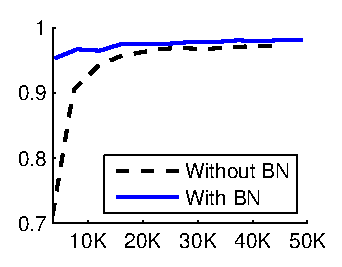
\includegraphics[width=0.28\columnwidth]{mnist.eps}
&
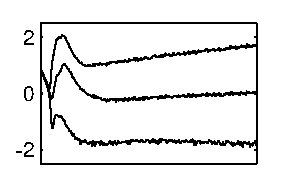
\includegraphics[width=0.35\columnwidth]{evo.eps}&
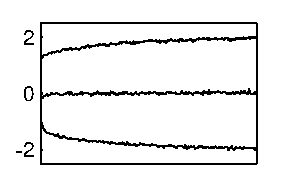
\includegraphics[width=0.35\columnwidth]{evo-bn.eps}\\
(a)&(b) Without BN&(c) With BN
\end{tabular} 
\caption{\em(a)} 
MNIST分别在有BN和没有BN训练的网络上的测试准确性,对比在不同数量的训练步骤。批量规范化网络帮助网络训练更快并且获得更高的准确性。
{\em(b, c)}在训练过程中,一个典型的sigmoid输入分布的演变,显示为{15\%,50\%,85\%}。批量规范化使得分布更加稳定并且减少了内部协变量转移。
\label{fig-mnist}
\end{figure}

图~\ref{fig-mnist}(a)显示的是随着训练的进展,两个网络对互斥测试数据的正确预测的分数。批量规范化的网络测试准确性比较高。为了研究为什么,在训练过程中,我们在原始网络$\norig$和批量规范化网络 $\ntrain$中研究了S形的输入(Alg.~\ref{alg-train})。在图~\ref{fig-mnist}(b,c)我们显示,对于来自每个网络的最后一个隐藏层的一个典型激活,其分布如何演变。原始网络中的分布随时间在它们的平均值和方差中改变显著,这使的后续层的训练变得复杂。相比之下,批处理规范化网络中的分布随着训练进展而更加稳定,这是有助于训练的。

\subsection{ImageNet 分类}
\label{sec-results}

我们将批量标准化应用于Inception网络\cite{inception}的一个新变体,在ImageNet分类任务\cite{imagenet}上进行了训练。这个网络有大量的卷积和池化层,一个预测图像类别超出1000个可能性的softmax层。卷积层使用ReLU作为非线性。\cite{inception}描述的网络主要的区别是5×5的卷积层由具有多达128个滤波器的3×3的两个连续卷积层代替。这个网络包含13.6*106个参数,除顶层softmax层之外,没有全连接层。更多的细节在附录中给出。我们在文章的其余部分将这个模型称为Inception。使用大小为32的小批量和具有动量的随机梯度下降的版本来训练模型。使用大规模的分布式架构进行训练(类似于\cite{dist-belief}).在训练过程中通过计算验证准确性$@1$来评估所有网络,即在互斥集上使用每个图像的单个裁剪来预测1000个可能性中的正确标签的概率。


\begin{figure*}
\centering
\begin{minipage}[b]{\columnwidth}
\begin{tabular}{@{}c@{}}
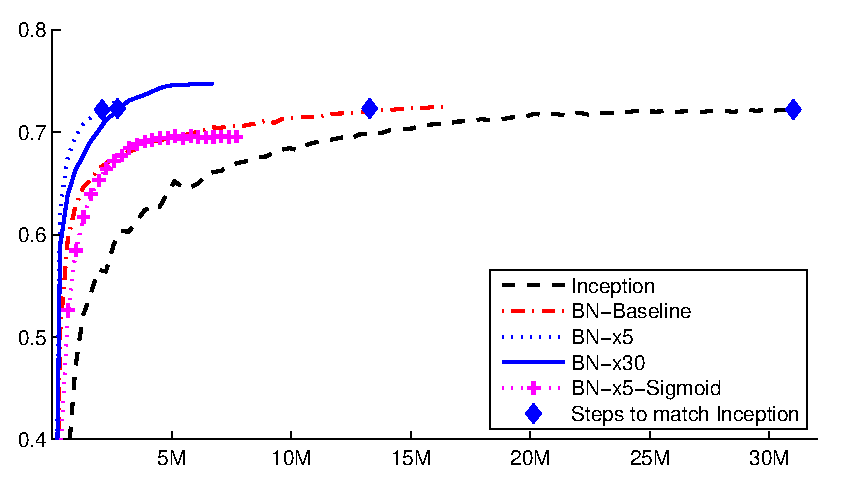
\includegraphics[width=\columnwidth]{inception-compare.eps}
\end{tabular} 
\caption{\em Single crop validation accuracy of Inception and its
  batch-normalized variants, vs. the number of training steps.  }
\label{fig-inception}
\end{minipage}
\qquad
%
\begin{minipage}[b]{0.9\columnwidth}
\begin{tabular}{@{} c | r  r  @{}}
\hline
Model & Steps to  72.2\% & Max accuracy \\ 
\hline
Inception& $31.0\mils$ & 72.2\%  \\
\sl BN-Baseline& $13.3\mils$ & 72.7\%  \\
\sl BN-x5& $2.1\mils$ & 73.0\%  \\
\sl BN-x30& $2.7\mils$ & 74.8\% \\
\sl BN-x5-Sigmoid&  & 69.8\%\\\hline
\end{tabular}
\caption{\em For Inception and the batch-normalized variants, the number of training steps required to reach the maximum accuracy of Inception (72.2\%), and the maximum accuracy achieved by the network.}
\label{fig-stats}
\end{minipage}
\end{figure*}

在我们的实验中,我们评估了规范化的Inception的几个修改。在所有情况下,批量规范化应用于每个非线性的输入,以卷积方式(如\ref{sec-conv}节所描述),同时保持架构的其余部分不变。

\subsubsection{加速BN网络}
\label{sec-accelerating}
简单地将Batch Normalization添加到网络并不能充分利用我们的方法。为此,我们进一步改变了网络及其训练参数,如下


{\em 增大学习率.} 在一个批量规范化模型,我们已经能够在较高的学习率下实现训练加速,而且没有不良的副作用 (Sec.~\ref{sec-lr}).

 {\em 去除Dropout.} 如~\ref{sec-regularizer}节所描述,批量规范化满足与Dropout相同的目标。从修改的BN-Inception中去除Dropout可加快训练,而切不会增加过拟合。
 
{\em 减少 $L_2$ 权重正则化.}在Inception里,模型参数上的损失控制过拟合,在修正的BN-Inception中,这个损失的权重减少了5倍。我们发现这提高了互斥验证数据的准确性。

{\em 加速学习速率衰减.} 
在训练Inception,学习率以指数方式衰减。因为我们的网络训练比Inception快,所以我们将学习速度降低了6倍.

{\em 去除本地响应规范化}   当Inception和其他网络 \cite{dropout} 从中受益时,我们发现使用批量规范化没有必要。

{\em 更彻底地改组训练样本.} 
我们启用了训练数据的内部改组,这防止了相同的样本总是出现在一个小批量中。这导致验证准确性提高约1\%,这与批量规范化作为一个正则化的观点一致(~\ref{sec-regularizer}节):当每次看到它不同的影响一个样本,我们的方法中固有的随机化应该是最有益的。

{\em 减少光度的扭曲.}
因为批量规范化网络训练更快,观察每个训练样本的次数更少,所以我们通过更少的扭曲关注更多的“真实”的图像。

\subsubsection{单个网络分类}
我们评估了以下网络,所有这些网络都训练了LSVRC2012训练数据,并对验证数据进行了测试:

\netw{Inception}: 在第\ref{sec-results}节开头描述的网络,训练初始学习率为0.0015。

\netw{BN-Baseline}: Inception与每个非线性之前的批量规范化相同。

\netw{BN-x5}: 在~\ref{sec-accelerating}节批量规范化的Inception和修改,初始学习率被提高了5倍到0.0075。与原始Inception相同的学习速率增加导致模型参数溢出。

\netw{BN-x30}: 类似于 \netw{BN-x5}, 但初始学习率为0.045(是Inception的30倍)。

\netw{BN-x5-Sigmoid}: 类似于 \netw{BN-x5}, 但是用sigmoid非线性 $g(t)=\frac{1}{1+\exp(-x)}$代替ReLU。我们也尝试用sigmoid去训练原始Inception,但该模型保持在相当于机会(chance)的准确性。

在图~\ref{fig-inception}我们显示网络的验证准确性,作为训练步骤数量的函数。Inception在训练步骤数量为$31\mils$之后准确达到72.2\%.图~\ref{fig-stats}显示,对于每个网络,达到相同72.2\% 精度所需的训练步骤的数量以及网络达到的最大验证精度和到达它的步骤数量。

仅通过使用批量规范化(\netw{BN-Baseline}),我们在不到一半的训练步骤中获得了Inception的准确性。通过使用~\ref{sec-accelerating}节中的修改,我们大大提高了网络的训练速度。BN-x5要达到Inception的72.2\%的准确率只需要比Inception少14倍的训练步骤.有趣的是,进一步提高学习率(\netw{BN-x30})导致模型开始训练有点慢,但允许其达到更高的最终精度。在训练步骤数量达到$6\mils$之后准确率达到74.8\%,在达到Inception72.2\%的准确率需要少于5倍的训练步骤。

我们还验证了内部协变量转移的减少允许使用sigmoid作为非线性时被训练的批量规范化的深度网络,尽管众所周知,训练这样的网络是很困难的。事实上,\netw{BN-x5-Sigmoid} 获得了69.8\%的准确率。没有批量规范化,具有sigmoid的Inception从未达到比$1/1000$更高的精度。

\subsubsection{集合分类}

\begin{figure*}[t!]
\centering
\begin{tabular}{c | r  r  r  r  r }
\hline
Model & Resolution & Crops & Models & Top-1 error & Top-5 error \\ 
\hline
{GoogLeNet ensemble} & 224 & 144 & 7 & - & 6.67\% \\
{Deep Image low-res} & 256 & - & 1 & - & 7.96\% \\
{Deep Image high-res} & 512 & - & 1 & 24.88 & 7.42\% \\
{Deep Image ensemble} & variable & - & - & - & 5.98\% \\
{BN-Inception single crop} & 224 & 1 & 1 & 25.2\% & 7.82\% \\
{BN-Inception multicrop} & 224 & 144 & 1 & 21.99\% & 5.82\% \\
{BN-Inception ensemble} & 224 & 144 & 6 & 20.1\% & {\bf 4.9\%}* \\
\hline
\end{tabular}
\caption{\em Batch-Normalized Inception comparison with previous state of the art on the provided validation set comprising 50000 images.
  *BN-Inception ensemble has reached 4.82\% top-5 error on the 100000 images of the test set of the ImageNet as reported by the test server. }
\label{fig-classification-comparison}
\end{figure*}

当前报道的ImageNet大规模视觉识别比赛的最佳结果是由传统模型的深图像集合\cite{deepimage}和\cite{msr}集合达到的。由ILSVRC 服务器评估后者显示前5误差率为4.94\%。我们在此得到一个前5 验证误差率为4.9\%和测试误差率为4.82\%(通过ILSVR服务器)。这改善了先前的最佳结果,并且超过根据的人类评估者的估计准确度\cite{imagenet}

%% jan16.pyplan/train_nbl0_lrmult6_wmp1
%% jan16.pyplan/train_lrmult6_wmp0_drop10
%% jan16.pyplan/train_lrmult6_wmp2_drop5
%% jan17.pyplan/train_nbl1_lrmult6_wmp1
%% jan17.pyplan/train_nbl1_lrmult6_wmp2
%% jan17.pyplan/train_nbl2_lrmult6_wmp1

对于我们的集合,我们使用6个网络。 每个都基于{\sl BN-x30},
通过以下一些修改:增加卷积层中的初始权重,使用Dropout(对原始Inception,Dropout为5\%或者10\%,对比40\%);和使用非卷积,每次激活使用模型的最后一个隐藏层进行批量规范化。每个网络大概在$6\mils$ 步骤后达到它的最大准确率。集合预测基于由构成网络预测的类概率的算术平均值。这个集合的细节和多向推理类似于\cite{inception}.

我们在图~\ref{fig-classification-comparison}中证明,批量规范化允许我们在ImageNet分类挑战基准上相当领先。

\section{结论}
我们提出了一个新的机制用来以显着的加速深度网络的训练。协变量转移会使机器学习系统的训练复杂化,我们的方法基于两个前提,1. 协变量转移关于整个系统的结论,也适用于子网络和层;2. 从网络的内部激活中去除协变量转移可以辅助训练。我们提出的方法强大之处在于规范化激活,并且将这种规范化结合在网络架构本身中。这确保了规范化可以与任何训练网络的优化方法合理融合。为了实现在深度网络训练中常用的随机优化方法,我们对每个小批量执行规范化,并且通过规范化参数反向传播梯度。批量规范化在每个激活只增加了两个额外参数,而这两个参数是为了保存网络的表述能力。我们提出了一个用于构建,训练和执行推理与批量规范化网络的算法。生成的网络可以用饱和非线性训练,可以容忍更大的学习率,并且可以减少或者减弱对Dropout正则化的使用。

仅仅将批量规范化添加到最先进图像分类模型中,就在训练中产生了实质的加速。通过进一步提高学习率,去除Dropout,并运用由批量规一化提供的其他修改,我们只用相对很少的训练步骤就达到了以前的最好结果 – 并且在单个网络图像分类上得到了更好的结果。此外,通过组合使用批量规范化训练的多个模型,我们在ImageNet上执行得比已知最好的系统好得多。

有趣的是,我们的方法与\cite{gulcehre}的标准层具有相似性,尽管这两种方法来自非常不同的目标,并且执行不同的任务。批量规范化的目标是在整个训练中实现激活值的一个稳定分布。在我们的实验中,我们在激活函数的非线性部分之前规范化一阶矩和二阶矩,这样做更容易导致稳定的激活函数值分布。相反,\cite{gulcehre}将标准化层应用于非线性部分的输出,这导致更稀疏的激活。在我们的大规模图像分类实验中,不管是否进行规范化,我们都没有观察到稀疏的非线性输入。批量规范化的其他显着区别特征包括,BN使用两个学习参数来保持网络的表达能力(标准化层不需要这样做,因为紧随其后就是被训练的线性变换,而这个线性变换可以提供必要的缩放与偏移)。除此之外BN的特性还包括其对卷积层的处理;其不依赖于小批量的确定性推理;以及其批量规范化网络中的每个卷积层。

在这项工作中,我们还没有探讨批量规范化潜在可能实现的全部可能性。我们未来的工作包括我们的方法到循环神经网络的应用\cite{pascanu-rnn}, 其中内部协变量转移和梯度的消失或发散可能特别严重,并且这将允许我们更彻底地测试规范化改善梯度传播的假设(在~\ref{sec-lr}节)。我们也计划研究一下,批量规一化是否可以帮助在传统意义上的域适应—比如,对群体均值和方差的重新计算(算法~\ref{alg-train})的规范化网络是否更容易适应新的数据分布。最后,我们相信对算法的进一步理论分析将允许更多的改进和应用。

\bibliography{bnicml}
\bibliographystyle{icml2015}


\section*{Appendix}
\subsection*{Variant of the Inception Model Used}
\begin{figure*}[b]
{\small
\begin{center}
  \begin{tabular}[H]{@{}|l|c|c|c|c|c|c|c|c|c|}
\hline
{\bf type} & {\bf \stackanchor{patch size/}{stride}} & {\bf \stackanchor{output}{size}} &
{\bf depth} & {\bf $\#1{\times}1$} & {\bf \stackanchor{$\#3{\times}3$}{reduce}} & $\#3{\times}3$ &
{\bf \stackanchor{double $\#3{\times}3$}{reduce}} & {\bf \stackanchor{double}{ $\#3{\times}3$}} & {\bf Pool +proj} \\
\hline\hline
convolution* & $7{\times}7/2$ & $112{\times}112{\times}64$ & 1 & & & & & & \\
\hline
max pool & $3{\times}3/2$ & $56{\times}56{\times}64$ & 0 & & & & & & \\
\hline
convolution & $3{\times}3/1$ & $56{\times}56{\times}192$ & 1 & & 64 & 192 & & &  \\
\hline
max pool & $3{\times}3/2$ & $28{\times}28{\times}192$ & 0 & & & & & & \\
\hline
inception (3a) & & $28{\times}28{\times}256$ & 3 & 64 & 64 & 64 & 64 & 96 & avg + 32  \\
\hline
inception (3b) & & $28{\times}28{\times}320$ & 3 & 64 & 64 & 96 & 64 & 96 & avg + 64 \\
\hline
inception (3c) & stride 2 & $28{\times}28{\times}576$ & 3 & 0 & 128 & 160 & 64 & 96 & max + pass through \\
\hline
inception (4a) & & $14{\times}14{\times}576$ & 3 & 224 & 64 & 96 & 96 & 128 & avg + 128 \\
\hline
inception (4b) & & $14{\times}14{\times}576$ & 3 & 192 & 96 & 128 & 96 & 128 & avg + 128 \\
\hline
inception (4c) & & $14{\times}14{\times}576$ & 3 & 160 & 128 & 160 & 128 & 160 & avg + 128 \\
\hline
inception (4d) & & $14{\times}14{\times}576$ & 3 & 96 & 128 & 192 & 160 & 192 & avg + 128 \\
\hline
inception (4e) & stride 2 & $14{\times}14{\times}1024$ & 3 & 0 & 128 & 192 & 192 & 256 & max + pass through \\
\hline
inception (5a) & & $7{\times}7{\times}1024$ & 3 & 352 & 192 & 320 & 160 & 224 & avg + 128 \\
\hline
inception (5b) & & $7{\times}7{\times}1024$ & 3 & 352 & 192 & 320 & 192 & 224 & max + 128 \\
\hline
avg pool & $7{\times}7/1$ & $1{\times}1{\times}1024$ & 0 & & & & & & \\
\hline
  \end{tabular}
\end{center}
}
\caption{Inception architecture}
\label{fig-arch}
\end{figure*}

Figure~\ref{fig-arch} documents the changes that were performed compared to the architecture with respect to the GoogleNet archictecture. For the interpretation of this table, please consult \cite{inception}. The notable architecture changes compared to the GoogLeNet model include:
\begin{itemize}
\item The 5${\times}$5 convolutional layers are replaced by two consecutive 3${\times}$3 convolutional layers. This increases the maximum depth of the network by 9 weight layers. Also it increases the number of parameters by 25\% and the computational cost is increased by about 30\%.
\item The number 28${\times}$28 inception modules is increased from 2 to 3.
\item Inside the modules, sometimes average, sometimes maximum-pooling is employed. This is indicated in the entries corresponding to the pooling layers of the table.
\item There are no across the board pooling layers between any two Inception modules, but stride-2 convolution/pooling layers are employed before the filter concatenation in the modules 3c, 4e.
\end{itemize}
Our model employed separable convolution with depth multiplier $8$ on the first convolutional layer. This reduces the computational cost while increasing the memory consumption at training time.


\end{document}
